\subsection{Vergleich zum O(1)-Scheduler}\label{s:compO1}
In den letzten Jahren ist der Anteil an Nutzern, die Linux als Desktop - Version einsetzen stetig gestiegen. Daher war es auch an der Zeit den CPU - Scheduler hinsichtlich Interaktivität zu verbessern. Unter anderem diesen Ansatz verfolgte Ingo Molnár mit der Entwicklung des O(1) - Schedulers. Laut \cite{papercomparison} haben Studien gezeigt, dass in Desktop - Umgebungen die Antwortzeit des Systems wichtiger bewertet wird als der Durchsatz. Für den Betrieb von interaktiven Anwendungen wird demnach eine sehr niedrige Latenz benötigt. 

Folgender Abschnitt folgt den Erläuterung aus \cite{asilberschatz} und \cite{papercomparison}.
Im Vergleich zum CFS arbeitet der O(1) - Scheduler mit je einer Warteschlange (engl. \textit{run queue}) pro Prozessor. Dabei besteht jede dieser Warteschlangen aus einem aktiven und abgelaufenen (engl. \textit{expired}) Array. Der Scheduler wählt den nächsten Prozess aus dem aktiven Array mit der höchsten Priorität. Wenn es Aufgaben mit gleicher Priorität gibt, wird per Round - Robin ausgewählt. Die Arrays sind zweidimensional mit 140 Prioritätsleveln angeordnet. So gibt es für Realzeitaufgaben Prioritäten von 0 (hohe Priorität) bis 99 (niedrige Priorität). Die konventionellen, zeitgeteilten Prozesse befinden sich im Interval von 100 - 139 und bilden gleichzeitig die \textit{nice} - Werte von -20 bis 19 ab. Wenn das aktive Array leer ist, d.h. keine weiteren Aufgaben mehr wählbar sind, werden die Zeiger der Arrays getauscht und das aktive wird zum abgelaufenen und umgekehrt. Die statischen Prioritäten werden um dynamische ergänzt indem der O(1) - Scheduler mittels einem Timer die durschnittliche \textit{sleep} - Zeit misst und somit die Priorität im Array anpasst. Bei einem Ablauf einer Zeitscheibe eines Prozesses wird die dynamische Priorität erneut kalkuliert, sodass bei einem Wechsel der Arrayzeiger die Elemente im Array mit den angepassten Prioritäten eingeordnet sind. Um die Interaktivität zu verbessern, versucht dieser Scheduler die interaktiven Prozesse zu identifizieren und zu bevorzugen. Dies geschieht anhand eines heuristischen Deltas. Ist dieses kleiner oder gleich einem definierten Bonus, werden interaktive Aufgaben im aktiven Array gehalten obwohl das Zeitquantum schon abgelaufen ist.

Fairness Test:
misst scheduler genauigkeit im verteilen der cpu bandbreite über multiple processes
-> papeor: diskrete integralrechnung von PI 
benchmark besteht aus parentproc und N kindprozessen
	erst werden alle geforked und warten auf signal
	wenn signal kommt fangen kinder gleichzeitig an zu rechnen
	messung in nanosec, dauer wird aufgezeichnet
	
messung mit 8,16,24,32 kindern, jedes set gleichzueigt und 100 mal wdh.
intel proc mit 2.13 ghz, 2gb ram, linux 2.6.22 O(1) linux 2.6.24.2 CFS -> nur ein core enabled damit nur eine runqueue genutzt

resultate im bild -> 32 kinder
standardabweichung der verbauchten zeit für jedes kind zum complete ist bei O(1) höhre als CFS
O(1) manche	kinder sind schneller fertig als andere -> weite streuung der daten
CFS Daten sind knapper beisammen und konzentrierter beim durchschnittswert
zsfsg: cfs verteilt cpu zeit über jede task in einer faireren weise
gründe: CFS teilt time-slices in sehr genau granularität \& accounting ist in nanosec
\begin{figure}[h]
	\centering
	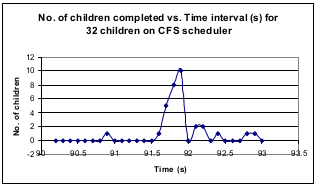
\includegraphics[width=0.45\textwidth]{pictures/fairness_32_cfs.png}
	\caption{Fairness-Messung für 32 Kinprozesse im CFS Scheduler.}
	\label{fig:fair_meas_cfs}
\end{figure}
\begin{figure}[h]
 	\centering
 	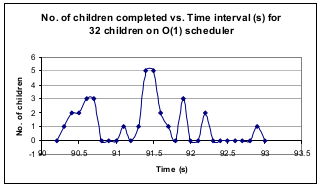
\includegraphics[width=0.45\textwidth]{pictures/fairness_32_O1.png}
 	\caption{Fairness-Messung für 32 Kinprozesse im O(1) Scheduler.}
 	\label{fig:fair_meas_o1}
\end{figure}

Interactive Test:
interaktiviät: scheduling latency o. jitter die in aufgaben unter versch. workloads präsentiert wird
Interbench -> versch. interactive taks mit background loads
misst die zeit zwischen dem anfragen der interactive taks der cpu ressource und wann sie sie tatsächlich bekommt
X.window simulation und audio, video, full load
3 tests je 100mal:	
  interact	background load
1 xwindow	audio 5 %
2 xwindow	vide 40 %
3 xwindow	full load 100 %
 
1. vergleiochsbenachmark: wieviele unbedeutende loops schafft das system in einer millisec -> constante in emulation
2. latenz zwischen start zeit des aufrufs des xwindow und wann es tatsächlich executing ist
	-> zeit die scheduler braucht um ressource zu alloc.
3. maximum und average /Mittelwert

Resultate:
CFS had neidriger latenz wenn wenig load, ansonsten höhere als O(1)
	allerdings ist latenz immer noch weit unter der menschl wahrnehmug, d.h. ein nutzer nimmt den unterschied nicht wahr (20-40ms braucht stimulus zum hirn)
CFS hat niedrigere Maximum werte in allen drei tests -> auch hier nicht wahrnehmbar
CFS lag time jeder task ist an period gebunden und O(1) jede prio hat auch gleiche base time slice

die bessere effizienz kann damit erklärt werden, weil fairer und cfs braucht keinen komplexen algo um interactive tasks zu identifizieren
\begin{figure}[h]
 	\centering
 	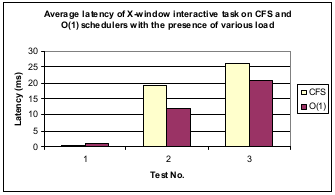
\includegraphics[width=0.45\textwidth]{pictures/avg_latency.png}
 	\caption{Durchschnittslatenz in CFS und O(1) Scheduler.}
 	\label{fig:avg_latency}
\end{figure}

\begin{figure}[h]
 	\centering
 	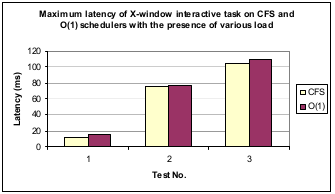
\includegraphics[width=0.45\textwidth]{pictures/max_latency.png}
 	\caption{Durchschnittslatenz in CFS und O(1) Scheduler.}
 	\label{fig:max_latency}
\end{figure}